Si può notare che le soluzioni aventi il minor numero di risorse utilizzate risultano essere la "Loop Unrolling Factor=2 Manual Solution" e la "Loop Unrolling Factor=2 Automatic Solution". In particolare, entrambe presentano, rispetto alla soluzione iniziale non ottimizzata, una diminuzione di circa il $64\%$ in corrispondenza delle LUT e del $55\%$ in corrispondenza dei FF. Inoltre, si può evidenziare un andamento crescente del numero dei FF al diminuire del periodo di clock in corrispondenza delle soluzioni hardware basate sulla tecnica dell'Operation Chaining. Infine, si possono notare i picchi di utilizzazione delle risorse in corrispondenza rispettivamente delle soluzioni hardware "Loop Unrolling Factor=2 Automatic and Partitioning Solution" e "Loop Unrolling Factor=4 Automatic and Partitioning Solution".

\begin{table}[H]
	\centering
	\begin{tabular}{|c|c|c|c|c|c|c|c|}
		\hline
		\textbf{Solution} & \textbf{LUT} & \textbf{LUTRAM} & \textbf{FF} & \textbf{BRAM} & \textbf{DSP} & \textbf{IO} & \textbf{BUFG} \\
		\hline
		Unopt & 275 & 32 & 160 & 0 & 2 & 71 & 1 \\
		Code Hoist & 270 & 32 & 134 & 0 & 2 & 71 & 1 \\
		Loop Fiss & 158 & 32 & 106 & 0 & 2 & 71 & 1 \\
		Unr2 Man & 98 & 0 & 72 & 1 & 2 & 71 & 1 \\
		Unr2 Auto & 98 & 0 & 72 & 1 & 2 & 71 & 1 \\
		Unr2 Auto Part. & 413 & 0 & 843 & 0 & 2 & 71 & 1 \\
		Unr4 Man & 159 & 0 & 147 & 1 & 2 & 71 & 1 \\
		Unr4 Auto & 145 & 0 & 93 & 1 & 2 & 71 & 1 \\
		Unr4 Auto Part & 1145 & 0 & 864 & 0 & 2 & 71 & 1 \\
		Op Chain 10ns & 275 & 32 & 160 & 0 & 2 & 71 & 1 \\
		Op Chain 9ns & 276 & 32 & 226 & 0 & 2 & 71 & 1 \\
		Op Chain 8ns & 276 & 32 & 226 & 0 & 2 & 71 & 1 \\
		Op Chain 7ns & 186 & 32 & 222 & 0 & 4 & 71 & 1 \\
		Op Chain 6ns & 186 & 32 & 241 & 0 & 4 & 71 & 1 \\
		Op Chain 5ns & 186 & 32 & 258 & 0 & 4 & 71 & 1 \\
		Op Chain 4ns & 188 & 32 & 376 & 0 & 4 & 71 & 1 \\
		Loop Pipe & 311 & 0 & 458 & 0 & 2 & 71 & 1 \\
		AXI & 739 & 0 & 699 & 0 & 0 & 93 & 1 \\
		\hline
	\end{tabular}
	\caption{Vivado Solutions Utilization Report [\#]}
	\label{tab:vivado-solutions-utilization-report}
\end{table}

\begin{figure}[H]
	\centering
	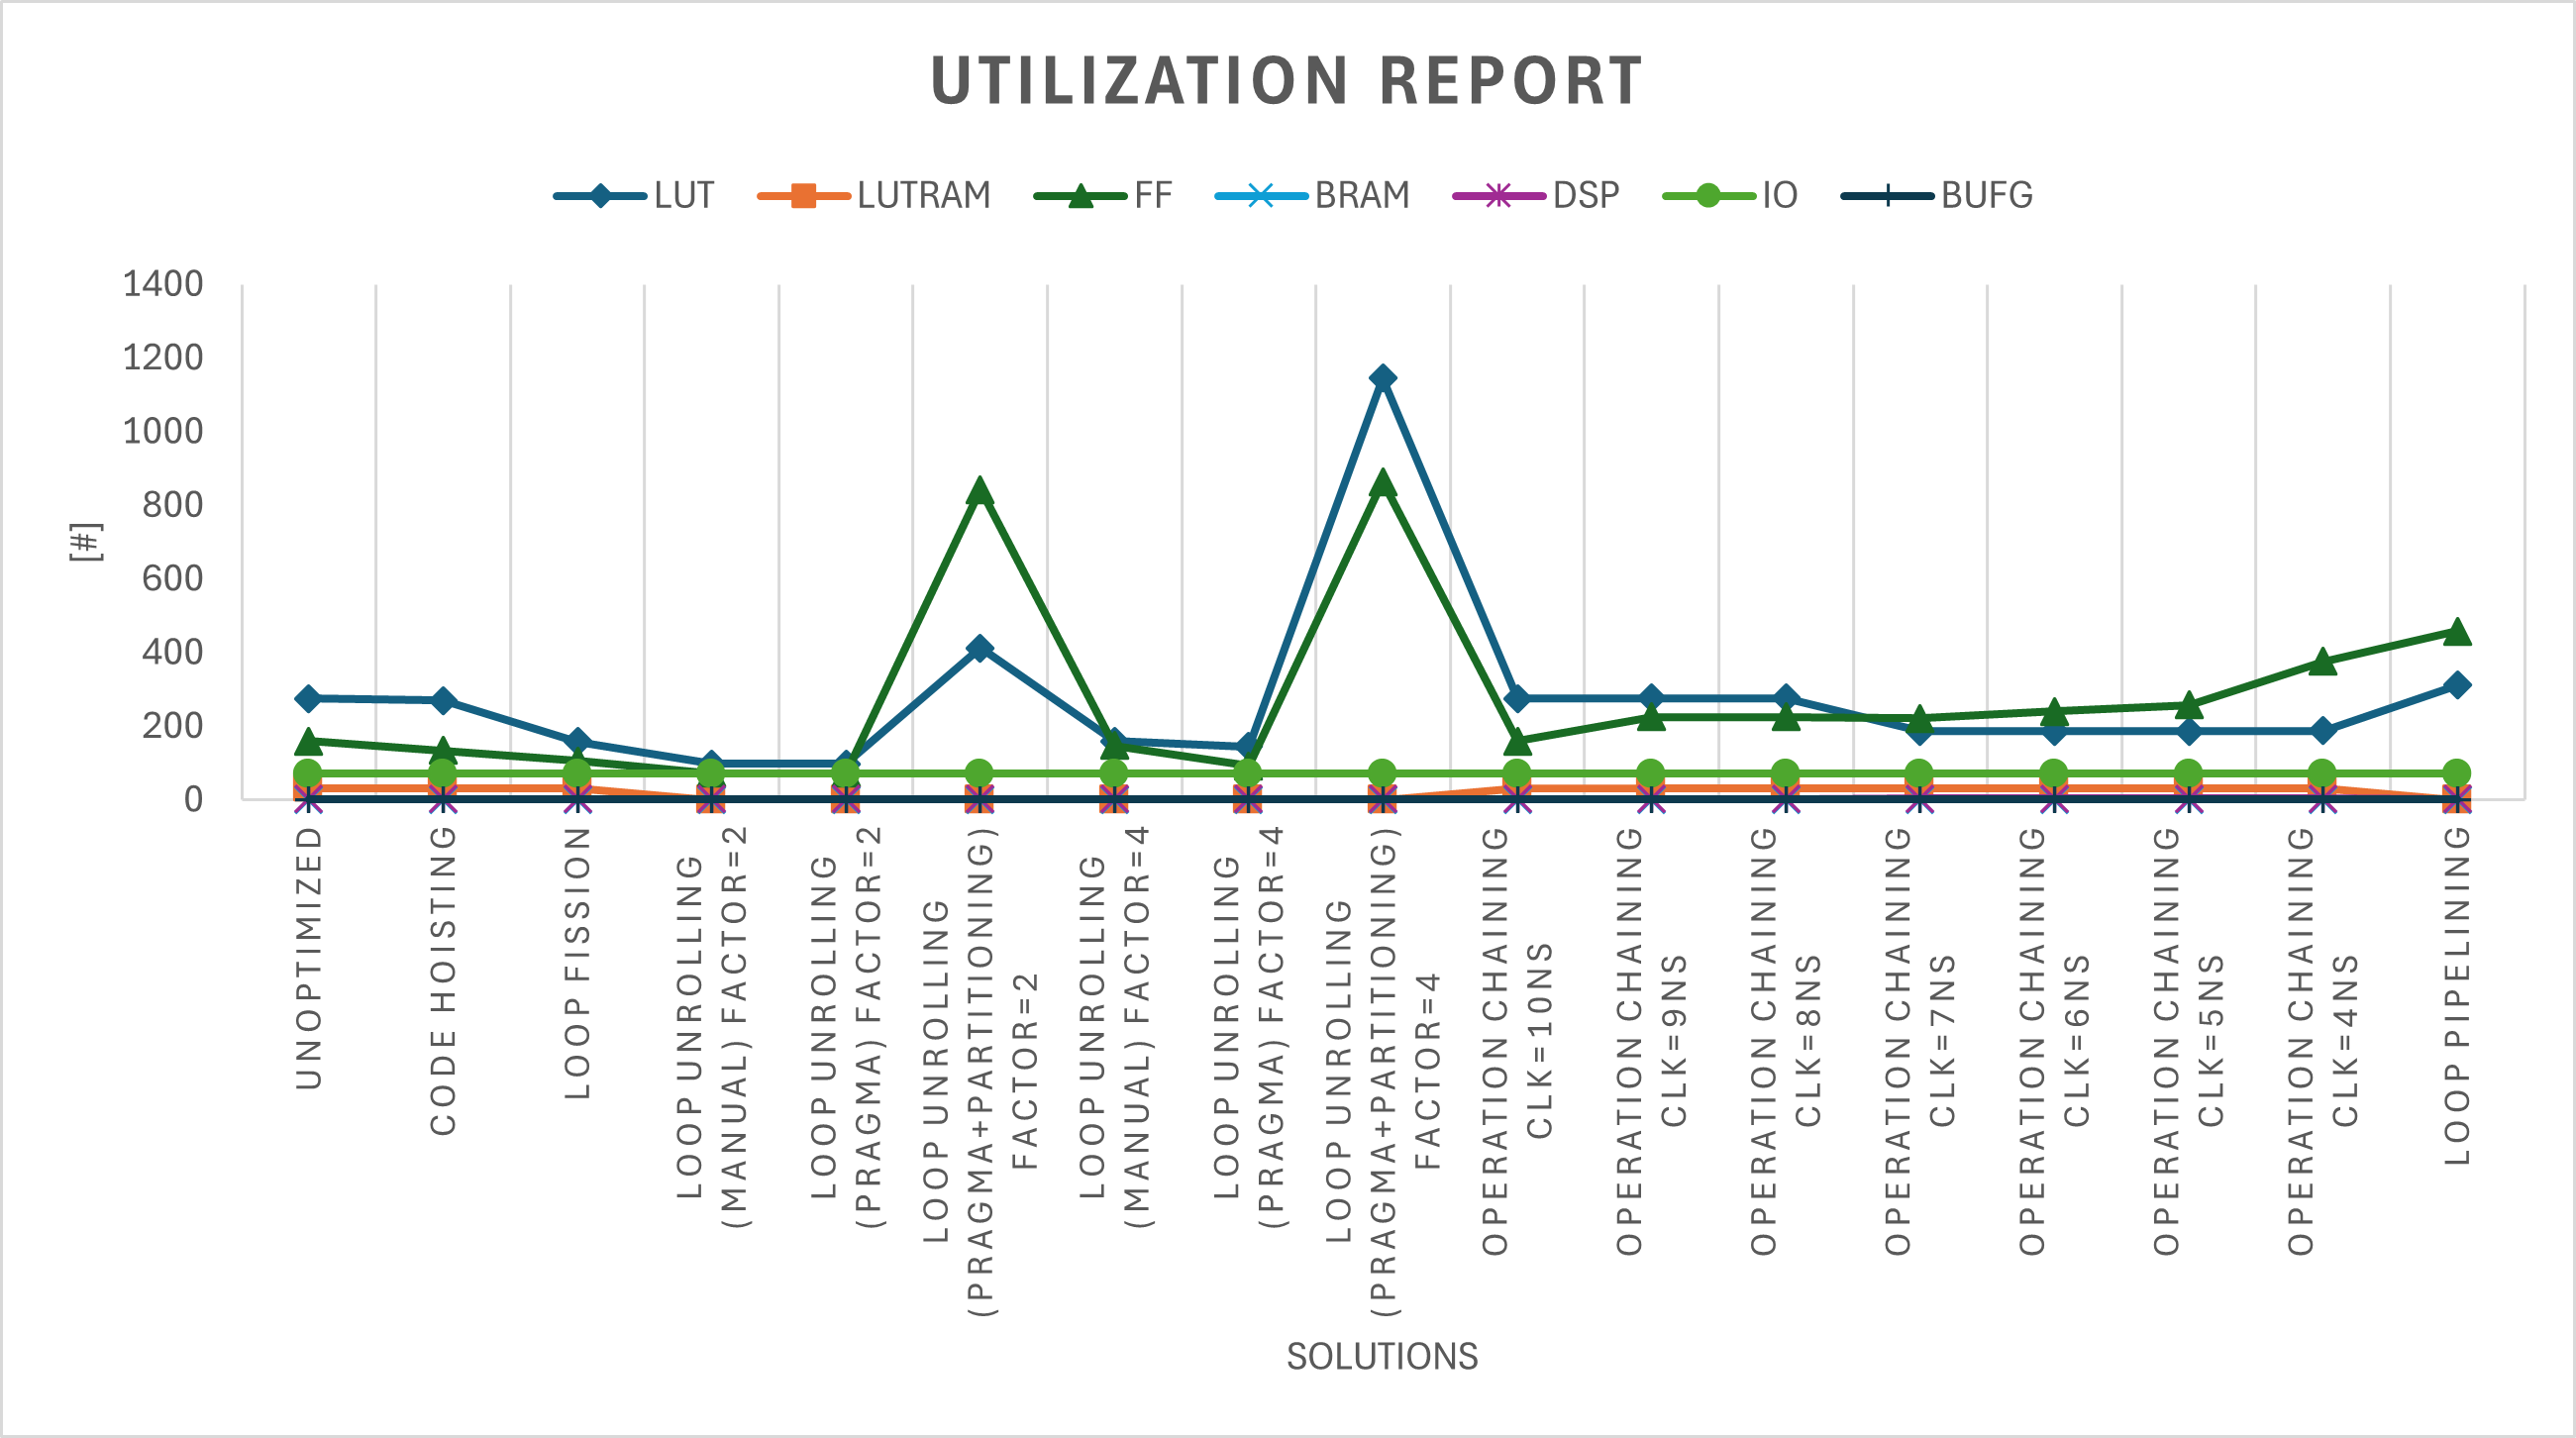
\includegraphics[width=0.6\textheight]{conclusions/utilization.png}
	\caption{Vivado Solutions Utilization Plot}
	\label{fig:vivado-solutions-utilization-plot}
\end{figure}


Per quanto riguarda la potenza dinamica totale e l'energia per singola operazione, i valori minori si hanno in corrispondenza delle soluzioni hardware basate sul loop unrolling di fattore pari a 2 manuale e automatico e di fattore pari a 4 automatico. Inoltre, si può evidenziare un andamento crescente al diminuire del periodo di clock in corrispondenza delle soluzioni hardware basate sulla tecnica dell'Operation Chaining. Infine, si può notare come i massimi valori si hanno in corrispondenza della soluzione AXI poiché, come precedentemente citato, si tiene conto della logica di controllo associata all'interfaccia.

\begin{table}[H]
	\centering
	\begin{tabular}{|c|c|c|c|c|c|c|c|}
		\hline
		\textbf{Solution} & \textbf{BRAM} & \textbf{Clock} & \textbf{Clocks} & \textbf{DSP} & \textbf{Logic} & \textbf{Set/}& \textbf{Data} \\
		& & \textbf{Enable} & & & & \textbf{Reset} & \\
		\hline
		Unopt & 0 & 0.454227469 & 1.215484925 & 0.335011806 & 0.921480532 & 3.57E-03 & 1.007059589 \\
		Code Hoist & 0 & 0.370487687 & 1.756788697 & 0.41467679 & 0.838255044 & 3.35E-03 & 1.381990616 \\
		Loop Fiss & 0 & 0.292603218 & 1.098937588 & 0.321194879 & 0.590288255 & 0.004160448 & 0.937705627 \\
		Unr2 Man & 1.250551548 & 0.096387172 & 0.900532817 & 0.268251897 & 0.260709843 & 0.003146866 & 0.423992984 \\
		Unr2 Auto & 1.240851358 & 0.082524632 & 0.960682868 & 0.272355421 & 0.266662013 & 0.00428147 & 0.425589533 \\
		Unr2 Auto Part & 0 & 0.325270201 & 2.352835611 & 0.263715046 & 0.575191109 & 0.007010513 & 0.750690058 \\
		Unr4 Man & 1.32976193 & 0.382625905 & 0.253616716 & 0.921033497 & 0.543549308 & 0.010887122 & 0.585376518 \\
		Unr4 Auto & 1.23103871 & 0.106978332 & 0.972227077 & 0.247065967 & 0.258892891 & 0.002585625 & 0.41881192 \\
		Unr4 Auto Part & 0 & 0.328624592 & 2.560390625 & 0.298048515 & 1.146363211 & 0.0030065 & 1.324957004 \\
		Op Chain 10ns & 0 & 0.455035944 & 1.215706812 & 0.343570428 & 0.925468281 & 0.00349783 & 1.014495501 \\
		Op Chain 9ns & 0 & 0.371109403 & 1.601127908 & 0.308091694 & 0.871003722 & 0.003504661 & 0.845550094 \\
		Op Chain 8ns & 0 & 0.432465255 & 1.790320966 & 0.364705513 & 1.03614782 & 0.003386509 & 1.085355412 \\
		Op Chain 7ns & 0 & 0.4179838 & 1.991891069 & 0.305155962 & 0.881534419 & 0.002575182 & 0.757947506 \\
		Op Chain 6ns & 0 & 0.367850007 & 2.092533279 & 0.244985771 & 0.788475969 & 0.00273619 & 0.666663051 \\
		Op Chain 5ns & 0 & 0.556948828 & 3.174162703 & 0.291668839 & 0.943421735 & 0.004532358 & 0.906153 \\
		Op Chain 4ns & 0 & 0.57213963 & 3.804846667 & 0.253423554 & 0.799402245 & 0.002476984 & 0.756326073 \\
		Loop Pipe & 0 & 0.196236724 & 1.778833685 & 0.814738101 & 1.275097136 & 0.012051522 & 1.206569896 \\
		AXI & 0 & 0.361682673 &	2.409646753 & 0 & 7.963255048 &	0.008282737 & 5.53872576 \\
		\hline
	\end{tabular}
	\caption{Vivado Solutions Dynamic Power Report [mW]}
	\label{tab:vivado-solutions-dynamic-power-report}
\end{table}

\begin{table}[H]
	\centering
	\begin{minipage}[t]{0.45\linewidth}
		\centering
		\begin{tabular}{|c|c|}
			\hline
			\textbf{Solution} & \textbf{Total Dynamic Power} \\
			\hline
			Unopt & 3.936829 \\
			Code Hoist & 4.765546 \\
			Loop Fiss & 3.24489 \\
			Unr2 Man & 3.203573 \\
			Unr2 Auto & 3.252947 \\
			Unr2 Auto Part & 4.274713 \\
			Unr4 Man & 4.026851 \\
			Unr4 Auto & 3.237601 \\
			Unr4 Auto Part & 5.66139 \\
			Op Chain 10ns & 3.957775 \\
			Op Chain 9ns & 4.000387 \\
			Op Chain 8ns & 4.712381 \\
			Op Chain 7ns & 4.357088 \\
			Op Chain 6ns & 4.163244 \\
			Op Chain 5ns & 5.876887 \\
			Op Chain 4ns & 6.188615 \\
			Loop Pipe & 5.283527 \\
			AXI & 16.28159297 \\
			\hline
		\end{tabular}
		\caption{Vivado Solutions Total Dynamic Power Report [mW]}
		\label{tab:vivado-solutions-total-dynamic-power-report}
	\end{minipage}
	\hfill
	\centering
	\begin{minipage}[t]{0.45\linewidth}
		\centering
		\begin{tabular}{|c|c|}
			\hline
			\textbf{Solution} & \textbf{Energy Single Operation} \\
			\hline
			Unopt & 39.36829 \\
			Code Hoist & 47.65546 \\
			Loop Fiss & 32.4489 \\
			Unr2 Man & 32.03573 \\
			Unr2 Prag & 32.52947 \\
			Unr2 Pragm Part & 42.74713 \\
			Unr4 Man & 40.26851 \\
			Unr4 Prag & 32.37601 \\
			Unr4 Pragm Part & 56.6139 \\
			Op Chain 10ns & 39.57775 \\
			Op Chain 9ns & 36.00349 \\
			Op Chain 8ns & 37.69905 \\
			Op Chain 7ns & 30.49962 \\
			Op Chain 6ns & 24.97947 \\
			Op Chain 5ns & 29.38444 \\
			Op Chain 4ns & 24.75446 \\
			Loop Pipe & 52.83527 \\
			AXI & 162.8159297 \\
			\hline
		\end{tabular}
		\caption{Vivado Solutions Energy Single Operation Report [pJ]}
		\label{tab:vivado-solutions-energy-single-operation-report}
	\end{minipage}
\end{table}

\begin{figure}[H]
	\centering
	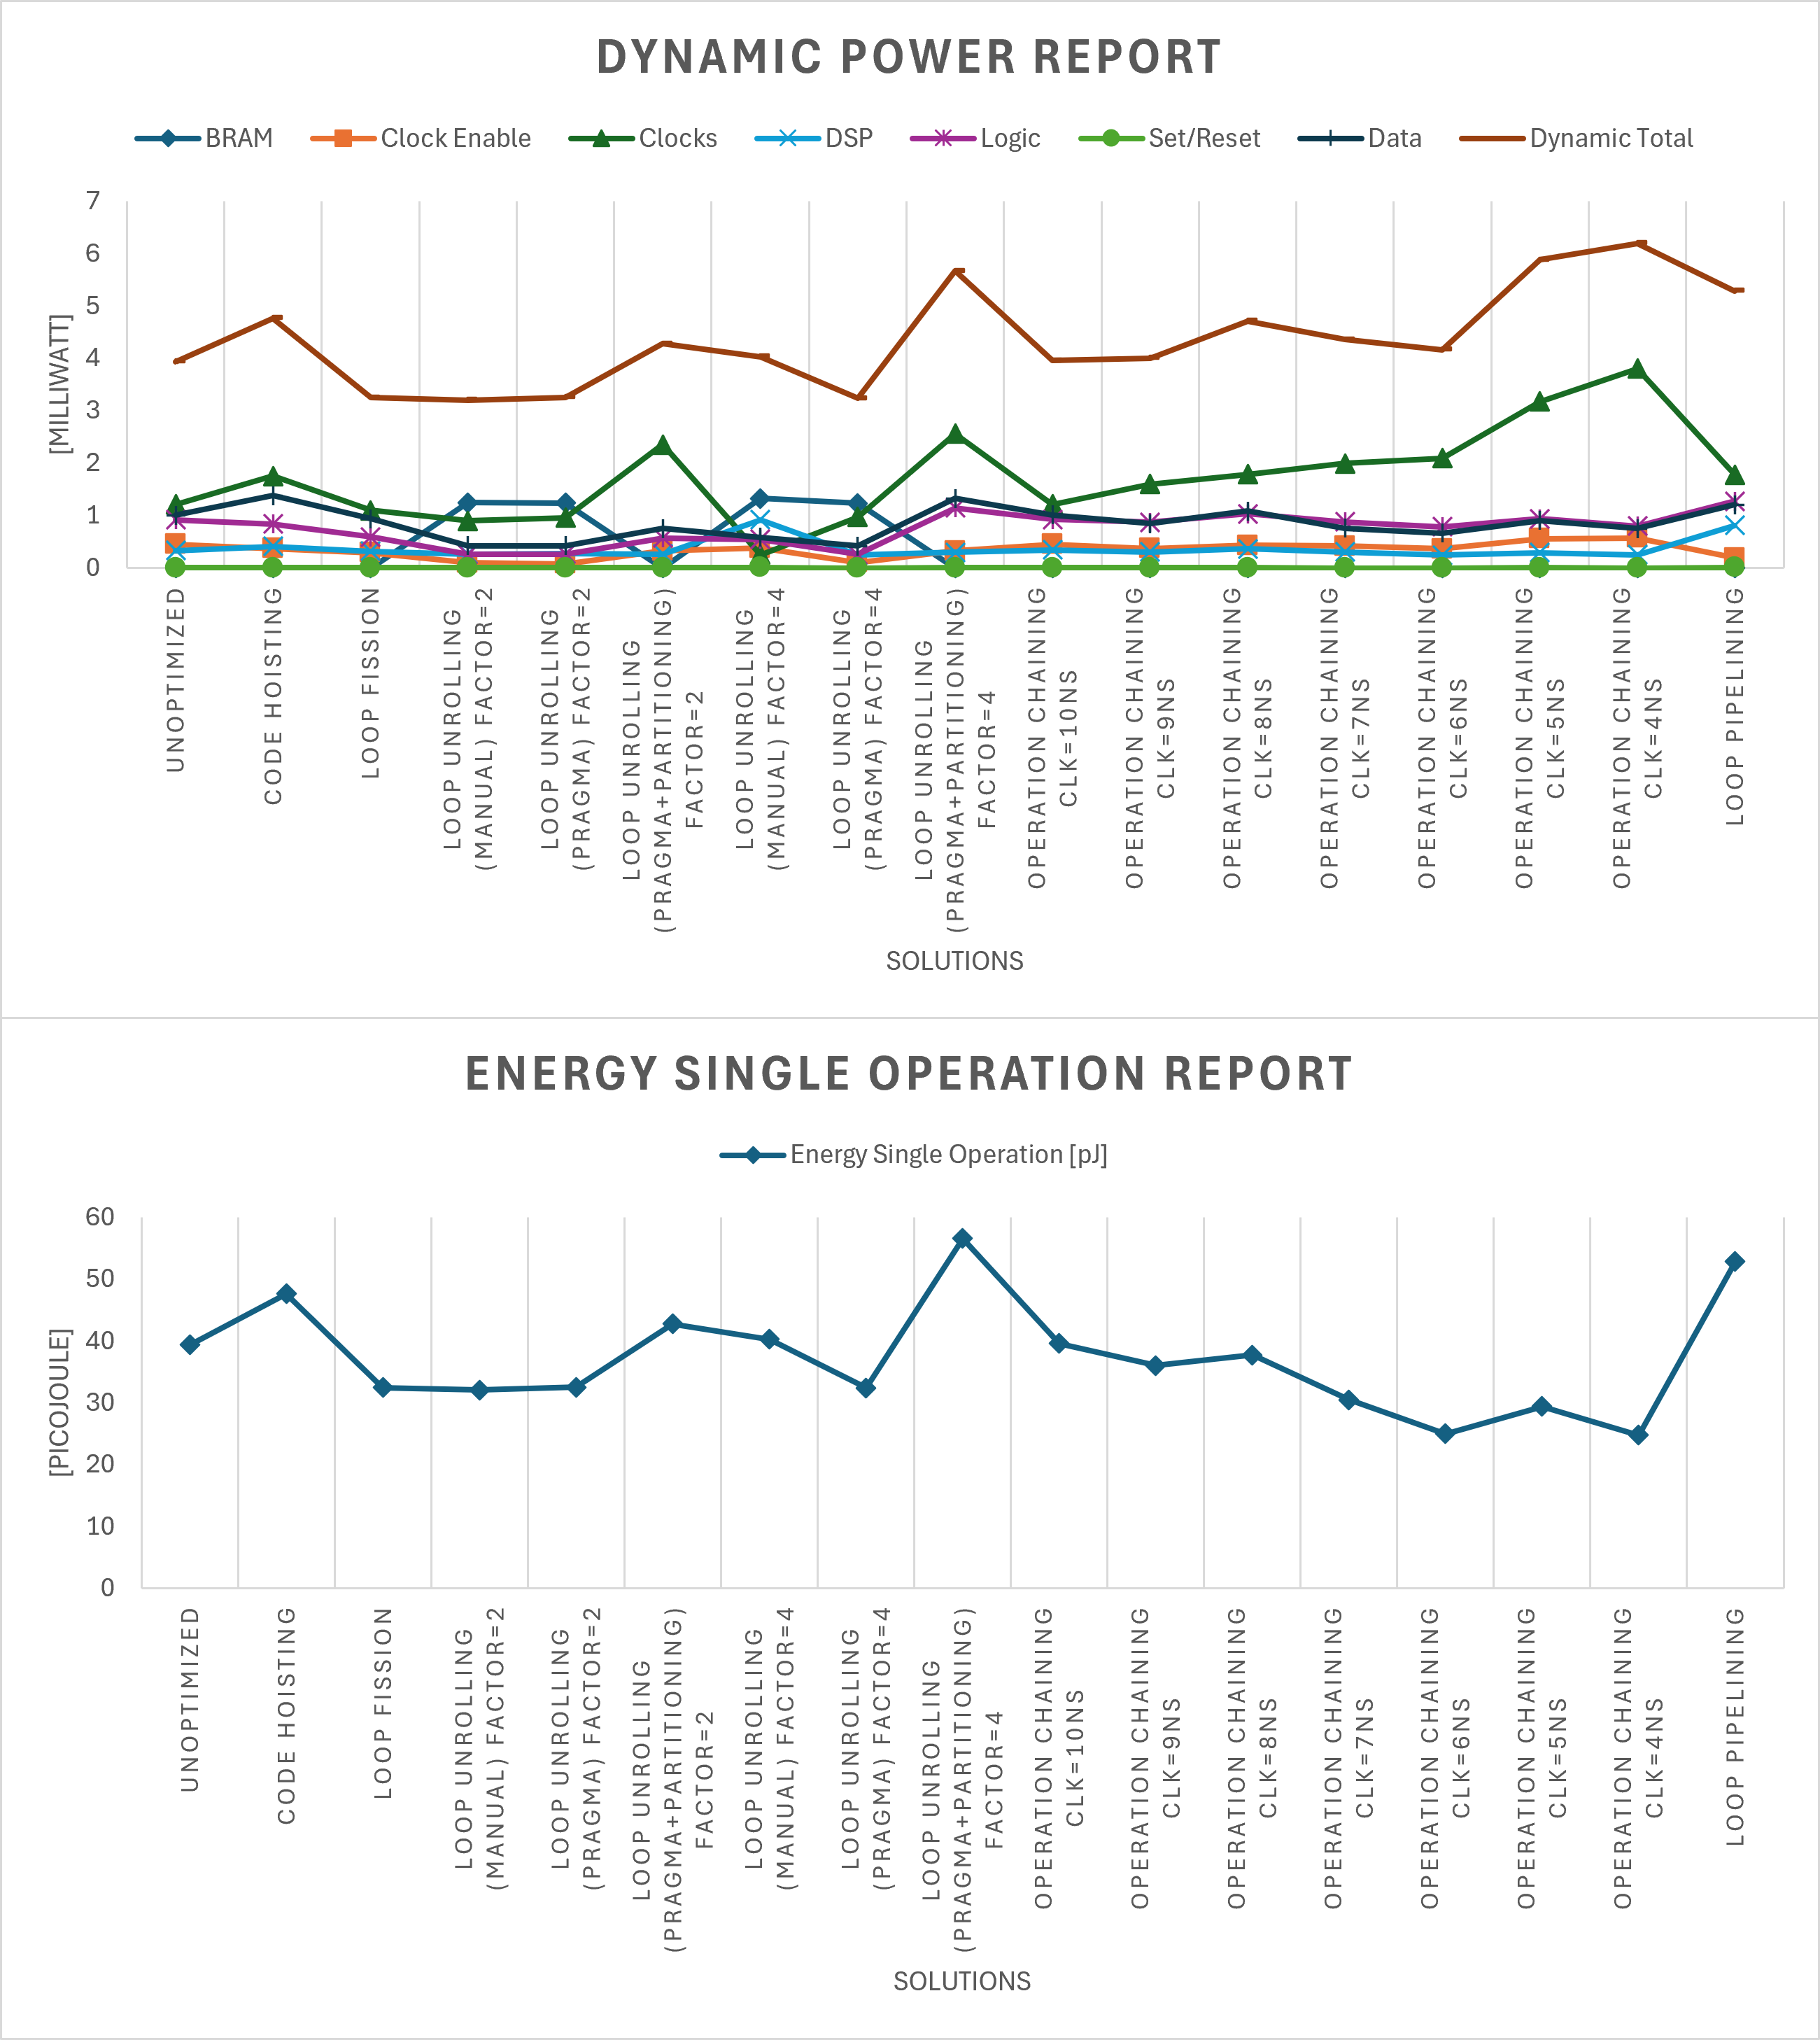
\includegraphics[width=0.7\textheight]{conclusions/powerreport.png}
	\caption{Vivado Total Dynamic Power and Energy Single Operation Plot}
	\label{fig:vivado-solutions-power-plot}
\end{figure}

Per quanto riguarda il report di timing, si può notare come il minor numero di cicli, utili per ottenere un risultato, si ha in corrispondenza della soluzione "AXI Solution" poiché, come già citato precedentemente, viene garantito un risultato parziale per ogni ciclo di clock a differenza delle altre solution che garantivano un risultato parziale con un numero di cicli nettamente maggiore (nel caso del "Loop Pipelining Solution", ad esempio, pari a 16). Tanto è vero che nella tabella, sotto allegata, in corrispondenza di "AXI Solution" il numero di cicli è pari a 1. Inoltre, si può evidenziare un andamento crescente al diminuire del periodo di clock in corrispondenza delle soluzioni hardware basate sulla tecnica dell'Operation Chaining. In particolare, in corrispondenza di un clock pari a 4ns si ha la soluzione hardware che presenta il maggior valore di cicli.
\\
Riguardo, invece, la Maximum Clock Frequency, il massimo valore si ha in corrispondenza della soluzione "Operation Chaining clk=4ns Solution" che presenta un valore pari a circa $282 MHz$. In particolare, nel caso della tecnica Operation Chaining, al diminuire del periodo del clock il WNS diminuisce e la massima frequenza aumenta.

\begin{table}[H]
	\centering
	\begin{tabular}{|c|c|c|c|c|}
		\hline
		\textbf{Solution} & \textbf{Cycles} & \textbf{Clock Constraint} & \textbf{WNS} & \textbf{Maximum Clock}\\
		& [\#] & [ns] & [ns] & \textbf{Frequency} [MHz]\\
		\hline
		Unopt & 44 & 10 & 3.654 & 157.5795777\\
		Code Hoist & 43 & 10 & 3.074 & 144.3834825\\
		Loop Fiss & 67 & 10 & 3.464 & 152.998776\\
		Unr2 Man & 57 & 10 & 4.33 & 176.366843\\
		Unr2 Prag & 57 & 10 & 4.33 & 176.366843\\
		Unr2 Part & 66 & 10 & 3.469 & 153.1159087\\
		Unr4 Man & 59 & 10 & 4.257 & 174.1250218\\
		Unr4 Prag & 61 & 10 & 4.33 & 176.366843\\
		Unr4 Part & 59 & 10 & 3.097 & 144.8645516\\
		Op Chain 10ns & 44 & 10 & 3.654 & 157.5795777\\
		Op Chain 9ns & 55 & 9 & 3.06 & 168.3501684\\
		Op Chain 8ns & 55 & 8 & 2.277 & 174.7335314\\
		Op Chain 7ns & 66 & 7 & 1.33 & 176.366843\\
		Op Chain 6ns & 88 & 6 & 1.573 & 225.8866049\\
		Op Chain 5ns & 88 & 5 & 0.374 & 216.1694769\\
		Op Chain 4ns & 131 & 4 & 0.454 & 282.0078962\\
		Loop Pipe & 16 & 10 & 4.208 & 172.6519337\\
		AXI & 1 & 10 & 1.369 & 115.8614297\\
		\hline
	\end{tabular}
	\caption{Vivado Solutions Timing Report}
	\label{tab:vivado-solutions-timing-report}
\end{table}

\begin{figure}[H]
	\centering
	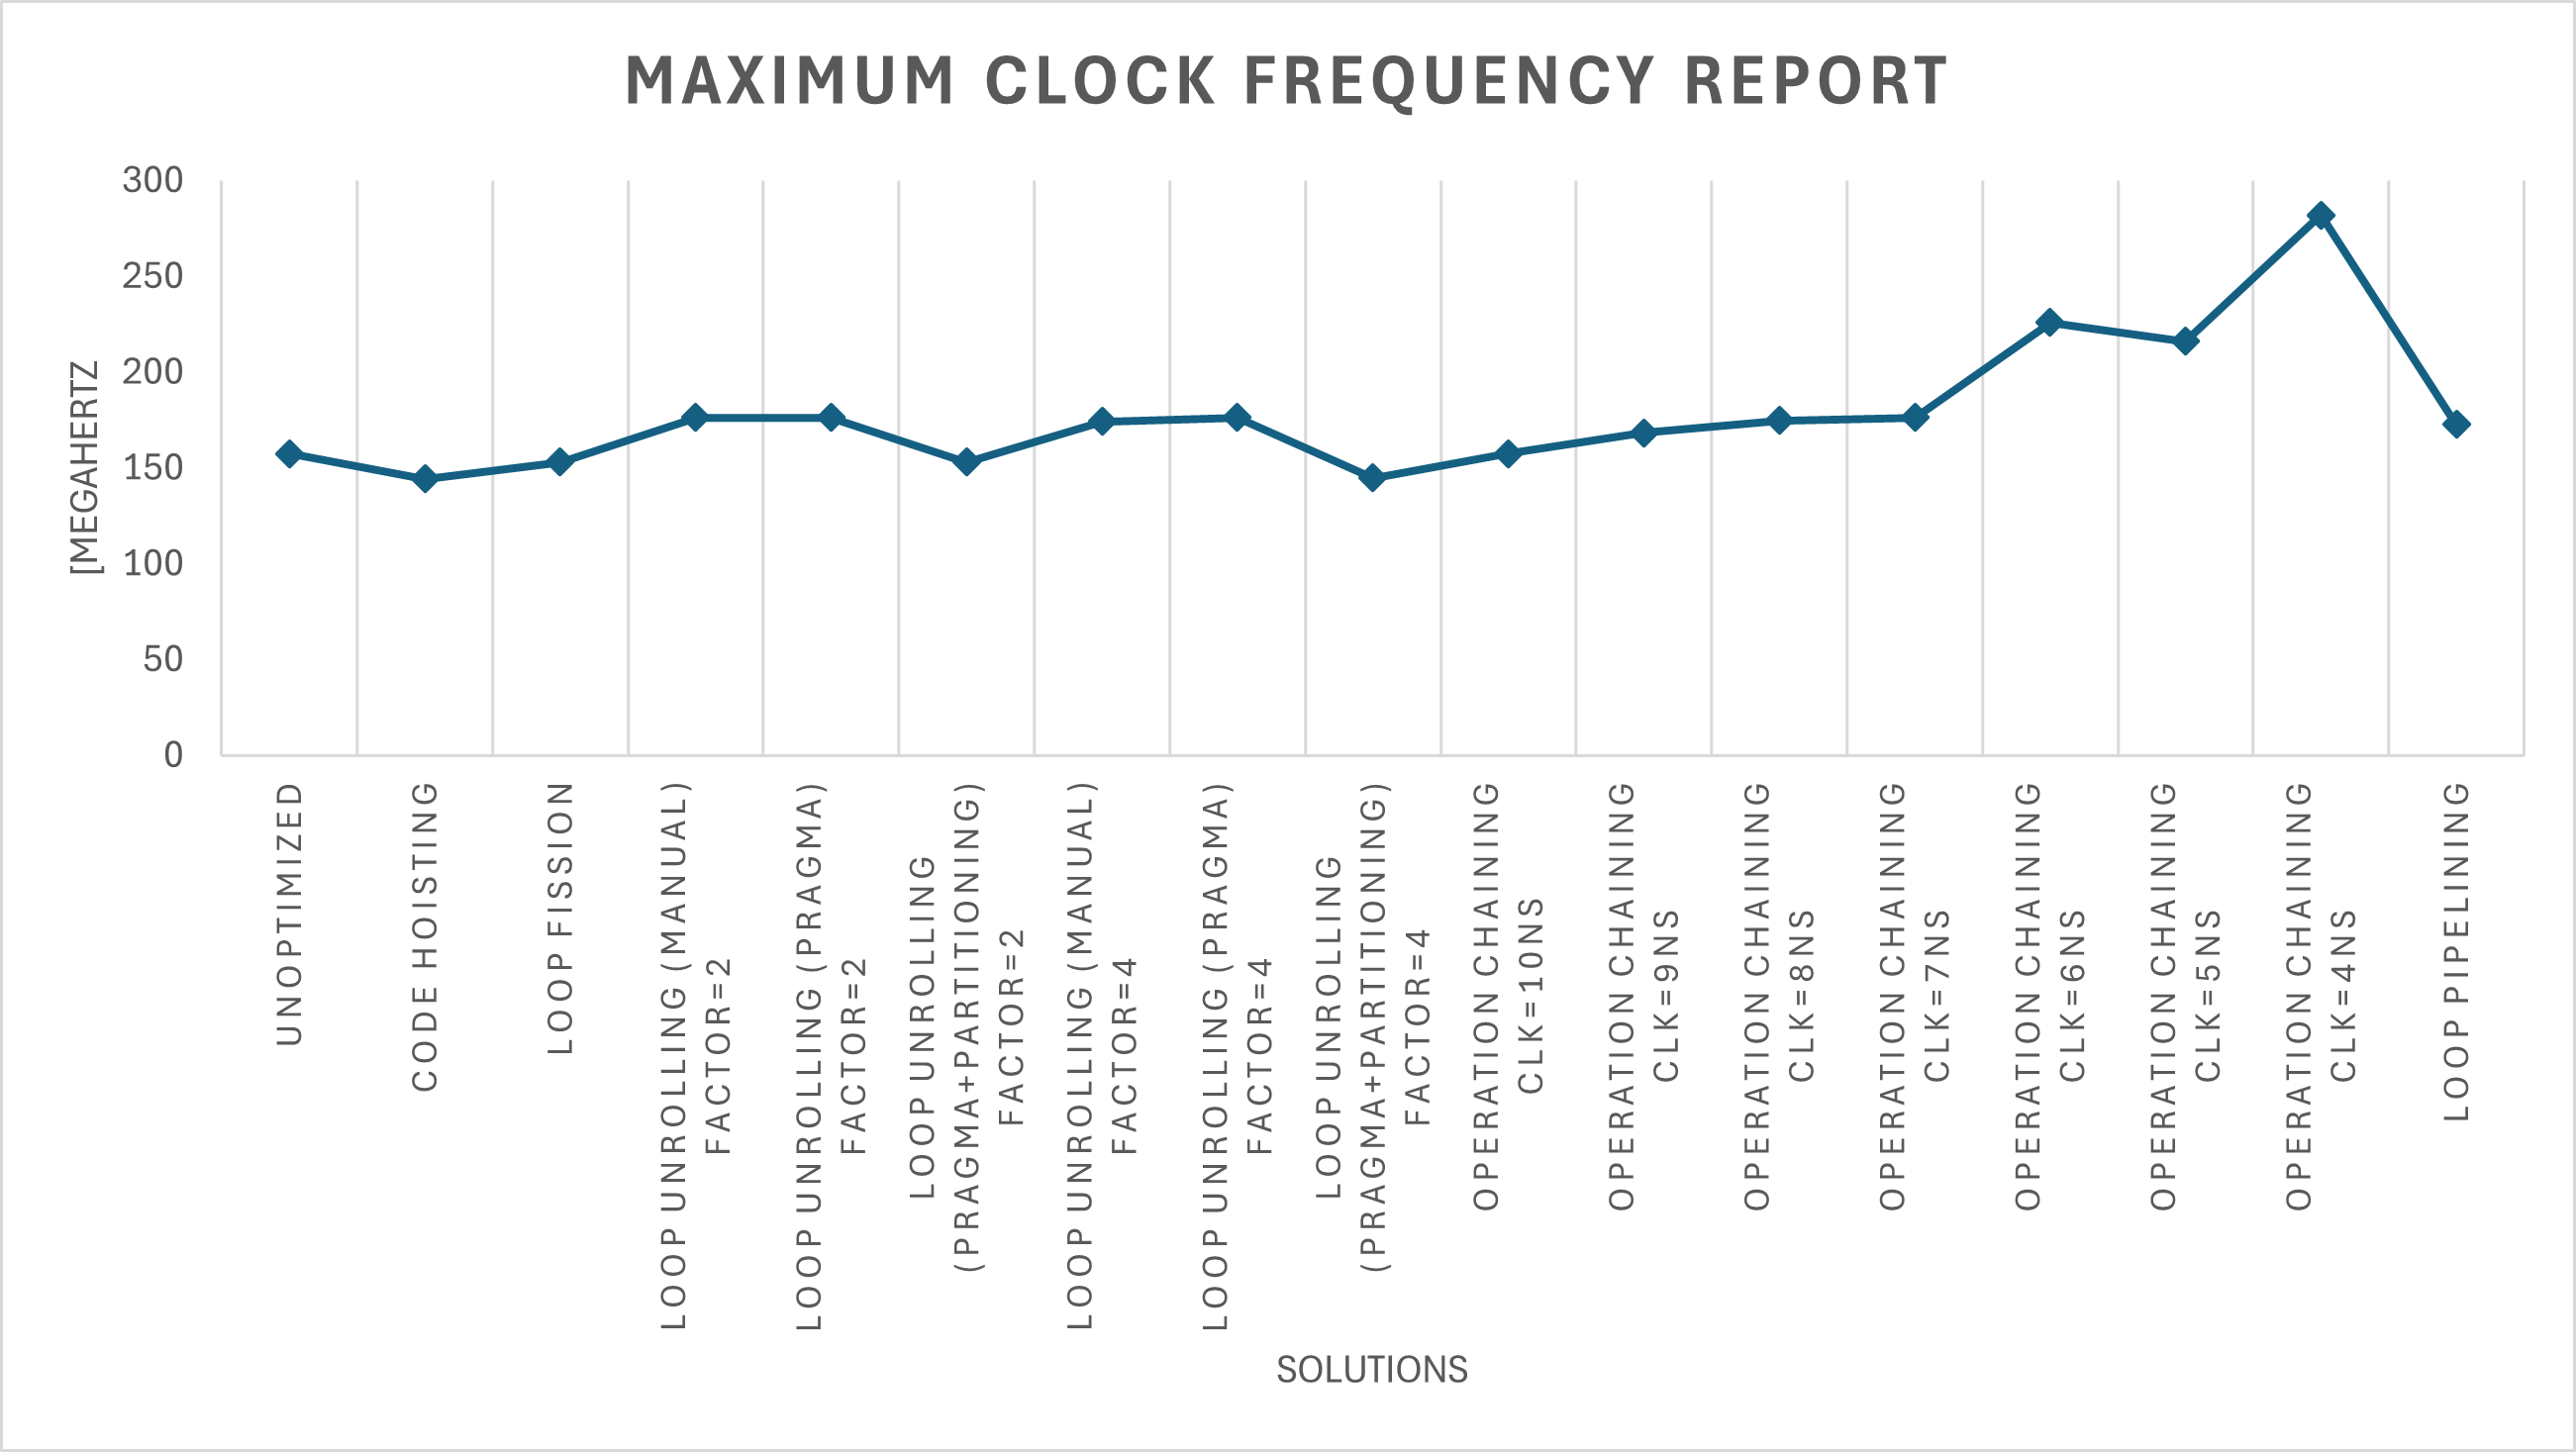
\includegraphics[width=0.7\textheight]{conclusions/frequency.png}
	\caption{Vivado Solutions Maximum Clock Frequency Plot}
	\label{fig:vivado-maximum-clock-frequency-plot}
\end{figure}

Tenendo conto delle analisi e dei confronti effettuati, si possono evidenziare alcune tecniche che presentano dei trade-off interessanti. In particolare, per quanto riguarda la tecnica dell'Operation Chaining, come già precedentemente citato, il periodo di clock ottimale è pari a 7ns. Infatti, confrontandola con la soluzione iniziale non ottimizzata, in corrispondenza di tale soluzione hardware si ha un leggero incremento del numero di cicli ma allo stesso tempo presenta un aumento della Maximum Clock Frequency e una diminuzione delle risorse utilizzate. Ovviamente bisogna anche tenere presente di un leggero aumento della potenza dinamica totale e dell'energia per singola operazione. Bisogna notare che una soluzione migliore rispetto a quella appena citata si ha in corrispondenza delle "Loop Unrolling Factor=2 Manual Solution" e "Loop Unrolling Factor=2 Automatic Solution". Tanto è vero che esse presentano, rispetto alla soluzione iniziale non ottimizzata, una diminuzione notevole delle risorse, una diminuzione della potenza dinamica totale e dell'energia per singola operazione e un aumento della Maximum Clock Frequency. Bisogna notare, però, che in corrispondenza di tali soluzioni si ha un leggero aumento del numero di cicli utili per ottenere un risultato. Ovviamente, nel caso in cui si debba ottenere il minor numero di cicli, bisognerebbe scegliere, come già precedentemente citato, la soluzione basata su AXI poiché permette di avere in uscita un risultato parziale per ogni ciclo di clock. Ad ogni modo, si avrebbe, in corrispondenza di tale soluzione hardware, un aumento dell'utilizzazione delle risorse, un aumento della potenza dinamica totale e dell'energia per singola operazione dovuti alla logica di controllo associata allo standard.